\section{Introduction}
\label{sec:intro}

Retrieval-augmented generation (RAG)~\citep{lewis2020rag} now powers
deployed systems across medical QA, legal research, and customer
support, yet many papers still evaluate faithfulness with a narrow
template: one retriever, one generator, one scorer, one threshold, and
one benchmark. That template is convenient, but it
\emph{under-identifies} the claim. A result that looks decisive in one
generator/retriever/scorer cell can change sign, shrink, or become a
deployment tradeoff under an equally defensible audit choice.

The trigger for this paper is a previously published refinement-paradox
claim of the form ``improving per-passage retrieval reduces answer
faithfulness.''\footnote{Cited at submission as a public claim; the
preprint reference is omitted here for double-blind review and will
be added on acceptance.} The headline was interesting enough to
audit, but it does not survive the controls reported here. At scale,
the original SQuAD generator-7B contrast shrinks to
$0.661 / 0.650 / 0.661$ across no-refinement, aggressive-refinement,
and gated-refinement conditions; a matched-similarity intervention on
context coherence is null; threshold-transfer cells change sign; and
a cost-aware head-to-head produces no dominating system.

The audit reframes the original headline as a stronger
methodological result. The problem is not that a coherence hypothesis
``failed''; the problem is that single-cell RAG faithfulness numbers
hide too many degrees of freedom. The empirical results in this paper
are not independent anecdotes: each one corresponds to an axis that a
RAG faithfulness claim must disclose.

The positive contribution is \textbf{ControlledRAG}: a reusable audit
checklist and prescriptive minimum reporting standard for RAG
faithfulness claims. ControlledRAG is not a new retriever, not a new
faithfulness metric, and not a method leaderboard. It asks authors to
vary or explicitly hold fixed seven axes---generator, retriever,
context structure, scorer, human calibration, threshold transfer, and
cost---so reviewers can tell whether a claim is robust or merely a
metric, retriever, generator, threshold, or cost artifact.

\paragraph{Contributions.} We make four contributions, mapped to
the seven-axis standard.
(i)~\textbf{The standard itself} (\S\ref{sec:controlledrag}): a
seven-axis disclosure checklist for RAG faithfulness claims, with
one principle---each axis is a movable quantity that, if left
unreported, lets a reader substitute a different reasonable value
and reach a different conclusion.
(ii)~\textbf{A self-applied seven-axis audit}
(\S\ref{sec:matched_ccs}--\S\ref{sec:cost}) on a previously
published refinement-paradox claim, exercising every axis of the
standard.
(iii)~\textbf{Two completed adjudicated human-eval slices}
(\S\ref{sec:human_cal}): a typical-row calibration
($n{=}99$, $\kappa{=}0.774$) and a targeted disagreement slice
($n{=}100$, $\kappa{=}0.721$) that reach \emph{different} scorer
rankings; the slice-dependence is the load-bearing finding under
the human-calibration axis.
(iv)~\textbf{An anonymized review artifact} containing auditable
per-query CSVs, matched context pairs, both human-eval slices,
source traces, and analysis scripts.

\paragraph{Why NeurIPS.} ControlledRAG is methodological, not
NLP-specific. The under-identification phenomenon is a
measurement-theory issue for any LLM-judged evaluation: same fixed
generations, different reasonable scorers, different reported
contrasts. The seven-axis decomposition is the contribution. We
\emph{conjecture} the decomposition generalises to other
LLM-as-judge settings (summarisation faithfulness, code-execution
evaluation, chain-of-thought scoring); demonstrating that
generalisation is out of scope here.

\paragraph{Roadmap.} \S\ref{sec:bg} compresses related work.
\S\ref{sec:setup} describes the pipeline and audited cells.
\S\ref{sec:controlledrag} defines ControlledRAG.
\S\ref{sec:matched_ccs}--\S\ref{sec:cost} run the seven-axis audit.
\S\ref{sec:discussion} discusses what survives. \S\ref{sec:limits}
states limitations. The supplement contains pre-specification
(\S 1), per-seed and per-cell detail (\S 2--\S 9), the
context-conditioned NLI rescoring (\S 7), the completed
$n=99$ calibration (\S 12) and the completed $n=100$ targeted
disagreement evaluation (\S 13), the source trace (\S 14), and the
related-work positioning table (\S 16).

\section{Background and Related Work}
\label{sec:bg}

A standard RAG system~\citep{lewis2020rag,gao2024ragsurvey} threads a
dense retriever~\citep{karpukhin2020dpr,xiong2024embedder}, an optional
reranker~\citep{nogueira2019passage}, an optional refinement step
(e.g., \citet{xu2024recomp}), and a generator. The implicit assumption
is that better local retrieval yields more faithful answers globally.
Decoder-side correctors take a different position:
Self-RAG~\citep{asai2024selfrag} retrains the generator to emit
reflection tokens, and CRAG~\citep{yan2024crag} adds a retrieval
evaluator that triggers web search; both pay latency cost.
RAPTOR~\citep{raptor2024} clusters retrieved passages into a tree and
retrieves from both leaves and LLM-summarised internal nodes
(\S\ref{sec:cost}). Faithfulness is typically scored with NLI-style
support metrics or LLM
judges~\citep{honovich2022true,laban2022summac,es2024ragas},
occasionally with human annotation. Recent evaluation frameworks
(ARES~\citep{saadfalcon2024ares}, RAGChecker~\citep{ru2024ragchecker},
RAGTruth~\citep{niu2024ragtruth}, MIRAGE~\citep{park2025mirage},
FaithJudge~\citep{tamber2025faithjudge}) supply judges, corpora, or
benchmark suites; ControlledRAG is the disclosure layer around them.
Discourse coherence has a long history in classical
generation~\citep{li2014coherence} but has not been quantified as a
deployment-time RAG signal (further coherence references in
supplement \S 16).
\citet{shi2023large} and \citet{liu2024lostmiddle} document
distraction by irrelevant context and lost-in-the-middle behaviour
respectively; we treat the Context Coherence Score (CCS) and
answer-bearing evidence presence as two complementary
context-structure variables to \emph{report} alongside per-passage
similarity, not as substitutes for human evaluation or cross-scorer
checks. The supplement reproduces a positioning table mapping each
prior framework to the audit axis it most directly engages.

\section{Setup and Audited Cells}
\label{sec:setup}

We hold the entire RAG pipeline fixed across audit experiments and vary
only the audit axis under test. The audited cells are deliberately
narrow---primarily short-answer extractive QA on SQuAD and PubMedQA
with $7$B-class generators---so that scorer, retriever, and generator
choices can be cleanly separated.

\paragraph{Datasets.} The matched-context, scaled, metric-fragility,
and span-control experiments use SQuAD~\citep{rajpurkar2016squad}; the
threshold-transfer and noise experiments additionally use
PubMedQA~\citep{jin2019pubmedqa}, HotpotQA~\citep{yang2018hotpotqa},
NaturalQuestions~\citep{kwiatkowski2019nq}, and TriviaQA. The long-form
stress test on QASPER and MS-MARCO is supplement-only and not treated
as broad generalization evidence (\S\ref{sec:limits} and supplement).

\paragraph{Pipeline.} Embeddings come from
\texttt{sentence-transformers/all-MiniLM-L$6$-v$2$}; indexing uses
ChromaDB; refinement uses
\texttt{cross-encoder/ms-marco-MiniLM-L-$6$-v$2$}. Default chunk size is
$1024$ characters with $10\%$ overlap and default top-$k$ is $3$.
Generators are served via local Ollama (Mistral-$7$B,
Qwen$2.5$-$7$B). The matched-context audit also re-encodes the same
$200$ pairs with BGE-large and E5-large.

\paragraph{Conditions.} Three retrieval configurations act as
instruments for measuring the audit surface, not as systems to crown
a winner. We name them by function and (in parentheses) by the prior
naming convention: \textbf{no-refinement} (top-$k$ dense retrieval,
also called \emph{baseline}); \textbf{aggressive-refinement} (refine
every retrieved passage through sub-chunking and cross-encoder
selection; the prior-work name is \emph{HCPC-v$1$} and this is the
original failure-mode condition the published refinement paradox was
based on); and \textbf{gated-refinement} (a coherence-gated variant
with top-rank protection, a refinement cap, and merge-back; prior-work
name \emph{HCPC-v$2$}). Tables and section text use the functional
names on first reference and the short prior names thereafter.

\paragraph{Metrics.} Per-query \textbf{faithfulness} in the legacy
audit tables is the stored automated support score in $[0,1]$;
\textbf{hallucination} indicates score $<0.5$ unless a table states
another label. The frozen DeBERTa and \texttt{roberta-large-mnli}
scores are sentence-level zero-shot entailment-label proxies (answer
sentence classified against entailment / neutral / contradiction with
\texttt{hypothesis\_template="\{\}"}; the retrieved context is
retained in the per-row data but not consumed by either proxy). The
RAGAS-style judge is context-conditioned by construction: a local
Mistral-$7$B receives the question, retrieved context, and answer and
returns a support score on $[0,1]$. \textbf{Retrieval similarity} is
the mean cosine similarity between the query and each retained chunk.
\textbf{CCS} is the mean minus the standard deviation of off-diagonal
pairwise cosine similarities between retained chunk embeddings (same
embedder). The answer-span indicator is a lowercased,
punctuation-stripped lexical match of any normalised gold-answer
alias in the retrieved context.

\paragraph{Statistical protocol.} The matched-context test is
pre-specified with paired Wilcoxon and a $10{,}000$-resample
bootstrap CI on the mean paired difference; the scaled audit reports
seed-level paired Wilcoxon over five seeds; binary rates use Wilson
$95\%$ CIs. P-values outside the pre-specified matched test are
descriptive across multiple audit cells; we do not treat exploratory
$p<0.05$ rows as standalone discoveries. All audit cells, paired
contrasts, and per-query CSVs are in the anonymized review artifact.

\section{ControlledRAG: The Minimum Reporting Standard}
\label{sec:controlledrag}

\paragraph{ControlledRAG is a checklist.} A paper that makes a RAG
faithfulness claim fills in seven entries, one per axis, and a
reviewer reads those entries to decide whether the claim is
generator-universal, scorer-dependent, threshold-dependent, or
otherwise narrow. The reporting-checklist template ships with the
artifact as
\texttt{controlledrag\_reporting\_checklist.md} (a filled-in copy
for this paper is included; this is \emph{distinct} from the
mandatory NeurIPS paper checklist that ships at the end of the
submitted PDF). Each entry asks: what was held fixed, what was
varied, why this choice, and what is the known sensitivity to
alternative reasonable values? The checklist is not a leaderboard
rubric and does not score papers; it is a disclosure layer that a
reviewer can use to ask one targeted question per axis.

\paragraph{Why seven axes, not six or eight.} A movable degree of
freedom belongs on the checklist if leaving it unreported lets a
reader substitute a different reasonable value and reach a different
conclusion. The seven axes the checklist asks every RAG faithfulness
paper to report, with the overclaim each blocks, are:
(1)~\emph{generator} (model family, size, decoding, fixed vs.\
regenerated outputs) blocks generator-universal claims; (2)~\emph{retriever}
(embedder, index, reranker, refinement policy) blocks ``retrieval
quality'' as one variable; (3)~\emph{context structure} (CCS, answer
span, mean similarity) blocks CCS-as-oracle; (4)~\emph{scorer}
(scorer names, input format, thresholds, cross-scorer correlations)
blocks single-score claims (\S\ref{sec:metric_fragility});
(5)~\emph{human calibration} (label protocol, raters, agreement, and
scorer-alignment correlations on at least one typical-row slice
\emph{and} on any targeted disagreement-driven slice) blocks
treating any metric ranking as settled (\S\ref{sec:human_cal});
(6)~\emph{threshold transfer} (tuned $\tau$, tune dataset,
off-diagonal recovery table) blocks reusable-threshold claims
(\S\ref{sec:threshold_transfer}); (7)~\emph{cost} (per-condition
latency, indexing time, external-call assumptions, including
baselines) blocks leaderboards without cost (\S\ref{sec:cost}). Six
axes drop one of these movable quantities; eight start to
double-count (decoding is a generator subfield; index size is a
retriever subfield) without adding a new degree of freedom. The
remainder of the paper supplies a self-applied audit in which each
empirical cell motivates one axis.

\section{The Matched-Context Audit}
\label{sec:matched_ccs}

The matched-context audit asks the diagnostic question directly:
\emph{at fixed mean per-passage query--passage similarity, does higher
CCS predict higher faithfulness?} The null answer is not the end of the
analysis. It creates a constructive diagnostic question: what variables
distinguish answer support once mean similarity is fixed?

\paragraph{Construction.} For SQuAD with Mistral, we form $200$
HIGH/LOW pairs so that mean query--passage similarity is matched to
within $0.02$ ($0.4236$/$0.4215$) while CCS is large in HIGH and small
in LOW ($0.670$/$0.137$).

\paragraph{Result.} Table~\ref{tab:matched_ccs_main} reports the
pre-specified HIGH--LOW contrast. The mean paired difference is
$-0.002$, paired Wilcoxon $p = 0.628$, Cohen's $d_z = -0.017$,
$10{,}000$-resample bootstrap $95\%$ CI $[-0.022, +0.017]$. The HIGH
hallucination rate is also \emph{higher} than the LOW rate
($16.5\%$ vs.\ $9.0\%$). The pre-specified $H_1$
(HIGH$>$LOW faithfulness) is not supported in the audited cell. The
continuous mean contrast and the thresholded hallucination contrast
measure different parts of the score distribution, so a null mean can
coexist with threshold-sensitive tail differences. The matched test
rules out the simple HIGH-CCS-improves-faithfulness story in this
audited cell.

\begin{table}[!htb]
\centering
\caption{Matched-context audit on SQuAD/Mistral ($n{=}200$ pairs,
matched mean query--passage similarity).}
\label{tab:matched_ccs_main}
\footnotesize
\begin{tabular}{lcccc}
\toprule
Quantity & HIGH-CCS & LOW-CCS & Difference & Test \\
\midrule
Mean similarity & $0.4236$ & $0.4215$ & $+0.0021$ & matched by construction \\
Mean CCS        & $0.670$  & $0.137$  & $+0.533$  & --- \\
Faithfulness    & $0.636$  & $0.639$  & $-0.002$  & paired Wilcoxon $p=0.628$ \\
Hallucination   & $16.5\%$ & $9.0\%$  & $+7.5$ pp & McNemar $p=0.011$ \\
$95\%$ CI on faith diff & --- & --- & $[-0.022, +0.017]$ & $10{,}000$-resample bootstrap \\
\bottomrule
\end{tabular}
\end{table}

\paragraph{Span presence in matched contexts.} A lexical
gold-answer-string check finds the answer more often in LOW-CCS
contexts than HIGH-CCS contexts ($27.0\%$ vs.\ $17.0\%$, McNemar
$p=0.011$). The structural property captured by CCS is therefore not
the same as ``the retrieved context contains the answer''; the
lexical span check is a weak proxy because retrieved text can contain
the answer string while failing to support the generated answer.

\paragraph{Answer-span/control diagnostic.} A regression and
classification panel on the matched cell ($n=400$ contexts; full table
in supplement \S 3) shows that for continuous DeBERTa faithfulness,
answer-span presence is the strongest single predictor ($R^2$ ranking
$0.019 > 0.003 > 0.002$), while for binary hallucination AUROC, CCS is
the strongest single predictor ($0.639 > 0.586 > 0.531$). The joint
feature set has the highest score on both ($R^2 = 0.025$, AUROC
$= 0.643$). Span and CCS therefore diagnose complementary failure
modes; we do not claim a directional role for either, that span
subsumes CCS, or that CCS subsumes span.

\section{The Scaled Audit}
\label{sec:scaling}

The scaled audit asks the same headline question---does
aggressive-refinement (HCPC-v$1$) reliably hurt faithfulness on
SQuAD/Mistral?---at $n=2{,}500$ examples per condition with five
seeds, each analysed by paired Wilcoxon on $500$-pair contrasts.
Pooled means are $0.661 / 0.650 / 0.661$ for no-refinement /
aggressive-refinement / gated-refinement with overlapping Wilson CIs
on hallucination rate ($14.6\% / 14.7\% / 14.3\%$;
Table~\ref{tab:scaling_main}). One of five seeds reaches $p<0.05$
for the no-refinement$-$aggressive-refinement contrast (seed 44,
paired $p=0.008$); the other four yield $p \in [0.083, 0.234]$. The
gated$-$aggressive contrast reaches significance in $3$ of $5$ seeds
with small per-seed magnitude ($0.003$--$0.019$).

\begin{table}[!htb]
\centering
\caption{Scaled audit on SQuAD/Mistral, $n=2{,}500$ per condition,
pooled across five seeds. Conditions are functional names with prior
naming in parentheses.}
\label{tab:scaling_main}
\footnotesize
\begin{tabular}{lcccc}
\toprule
Condition & Faithfulness ($95\%$ CI) & Hallucination (Wilson) & Retrieval sim.\ & Refine rate \\
\midrule
no-refinement (baseline)        & $0.661 \, [0.655, 0.667]$ & $14.6\% \, [13.3, 16.0]$ & $0.532$ & $0.000$ \\
aggressive-refinement (HCPC-v$1$) & $0.650 \, [0.645, 0.656]$ & $14.7\% \, [13.4, 16.2]$ & $0.569$ & $1.000$ \\
gated-refinement (HCPC-v$2$)    & $0.661 \, [0.655, 0.667]$ & $14.3\% \, [13.0, 15.7]$ & $0.532$ & $0.705$ \\
\bottomrule
\end{tabular}
\end{table}

The originally published $n=30$ headline ($0.7995 \to 0.6407$ on
no-refinement vs.\ aggressive-refinement; see footnote 1) does not
survive at scale. The scaled contrast is small and seed-sensitive
and should not be cited as a broad refinement-hurts-faithfulness
claim. This is itself a ControlledRAG-style audit lesson: at $n=30$
the contrast looked clean enough to report as a phenomenon, but at
$n=2{,}500$ it does not.

\section{Fixed-Generation Metric Fragility}
\label{sec:metric_fragility}

This section is the core empirical pillar for the scorer axis. For the
scaled audit's $7{,}500$ Mistral rows, outputs are fixed before
rescoring, retrieval condition is fixed, and the only changed
component is the scorer. The three scorers are not on a common
numerical scale---two are legacy zero-shot label proxies that do not
consume the retrieved context, and the third is a context-conditioned
local judge---so raw score differences across scorers are not
interpreted as directly comparable causal estimates. To address the
scale concern, we standardize each scorer over the same fixed rows by
both z-scoring and rank-normalising before computing the paired
contrast. The important claim is that the sign, magnitude, and ranking
of the reported contrast remain scorer-sensitive on fixed generations
even after standardisation. We then run a compact second-generator probe (Qwen$2.5$, $n=100$
fixed contexts per condition, one model only; not a population-level
replication) and check whether the raw-contrast ordering is
preserved.

\begin{table}[!htb]
\centering
\caption{Fixed-generation metric fragility. Raw values are
no-refinement$-$aggressive-refinement score differences on each
scorer's native scale and \emph{are not directly comparable across
scorers}. Mistral z/rank columns standardize each scorer over the
same fixed rows before computing the paired contrast; bootstrap CIs
are in the supplement. The first two rows are legacy zero-shot label
proxies that do not consume the retrieved context (\S\ref{sec:setup});
the third is a context-conditioned local judge.}
\label{tab:metric_fragility_main}
\footnotesize
\begin{tabular}{lcccc}
\toprule
Scorer & Mistral raw & Mistral z & Mistral rank & Qwen$2.5$ raw \\
\midrule
Legacy DeBERTa proxy (no context) & $0.011$ & $0.071$ SD & $0.022$ & $0.015$ \\
Legacy \texttt{roberta-large-mnli} proxy (no context) & $0.032$ & $0.231$ SD & $0.062$ & $0.046$ \\
Context-conditioned RAGAS-style judge & $0.140$ & $0.337$ SD & $0.085$ & $0.134$ \\
\bottomrule
\end{tabular}
\end{table}

Cross-scorer Pearson correlations on the same fixed Mistral rows are
weak between the legacy DeBERTa proxy and the other two scorers
(DeBERTa vs.\ \texttt{roberta-large-mnli}: $r=0.259$; DeBERTa vs.\
RAGAS-style: $r=0.182$) and moderate between the
\texttt{roberta-large-mnli} proxy and the RAGAS-style judge
($r=0.674$); supplement \S 6 shows the same ordering on the Qwen$2.5$
second-generator probe. The two NLI-style rows are legacy zero-shot
entailment-label proxies (answer sentence as the sequence to be
classified, retrieved context not consumed); the RAGAS-style row is
context-conditioned by construction (the question, retrieved context,
and answer are all passed to a local Mistral-$7$B that returns a
support score with a short rationale). Scorer choice and scorer input
format are therefore an audit axis, not hidden implementation trivia.

\paragraph{Scorer input format is itself an audit axis.}
To make the input-format claim concrete, we rescore a balanced subset
of the same fixed-generation rows ($n=200$ paired queries per
condition, $n=600$ total) under a context-conditioned NLI calling
convention (premise $=$ retrieved context, hypothesis $=$ generated
answer sentence) for both DeBERTa-v$3$ and
\texttt{roberta-large-mnli}.
Figure~\ref{fig:metric_fragility_forest} reports the resulting
baseline$-$aggressive-refinement contrasts. Under context-conditioned
NLI the same two backbone models produce \emph{sign-flipped}
contrasts on the same fixed generations: the legacy and
context-conditioned bootstrap intervals are disjoint for both NLI
backbones. Passing the retrieved context as premise to the same
backbone weights changes the \emph{sign} of the reported contrast at
this audit cell.

\begin{figure}[!htb]
\centering
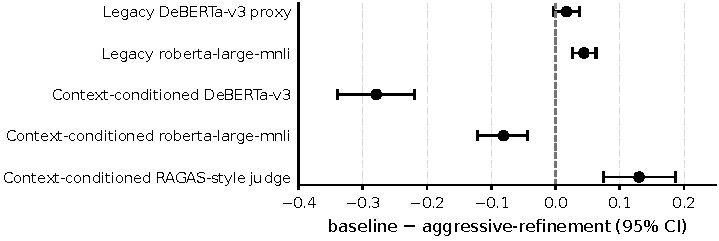
\includegraphics[width=0.68\linewidth]{figures/metric_fragility_forest.pdf}
\caption{Same fixed generations, same NLI backbones, sign-flipped
contrasts under different calling conventions
(baseline$-$aggressive-refinement on the $n=600$ balanced subset;
$10{,}000$-resample paired bootstrap $95\%$ CIs).}
\label{fig:metric_fragility_forest}
\end{figure}

\paragraph{Interpretation.} Among the seven axes audited here,
scorer choice is the largest movable quantity in the headline
number, and it remains movable after standardisation; under proper
context-conditioned NLI the two backbone NLI models produce
sign-flipped contrasts on the same fixed generations. The $n=99$ adjudicated calibration
(\S\ref{sec:human_cal_99}) shows overlapping bootstrap CIs across
scorers, so it does not settle a ranking either. Together these
findings make scorer choice an audit axis, not an implementation
detail: ControlledRAG requires at least two scorers, their input
format (whether retrieved context is consumed), and a cross-scorer
correlation to be reported. Scorer triangulation is not proof of
correctness; it discloses how much of the reported number is
scorer-dependent.

\section{Human Calibration: Two Slices, Different Scorer Rankings}
\label{sec:human_cal}

The human-calibration axis has two completed parts: the
\textbf{typical-row calibration} ($n=99$ stratified examples,
two passes plus adjudication) and the \textbf{targeted disagreement
slice} ($n=100$ examples ranked by scorer disagreement, two raters
plus adjudication). Both are load-bearing under ControlledRAG: the
first estimates scorer alignment on the typical row distribution,
the second stress-tests scorer alignment where automated scorers
most disagree. The two slices reach \emph{different} scorer
rankings; that slice-dependence is the load-bearing finding.

\subsection{Typical-row calibration ($n=99$).}
\label{sec:human_cal_99}

We sampled $99$ rows from the $7{,}500$ Mistral fixed-generation
audit, stratified across no-refinement / aggressive-refinement /
gated-refinement, and
applied a two-pass annotation protocol with three labels
(\texttt{supported}, \texttt{partially\_supported},
\texttt{unsupported}) plus an adjudication step. Annotators used only
the retrieved context. The two passes reach raw exact-match agreement
$0.919$ ($91/99$), Cohen's $\kappa = 0.774$, with adjudicated
distribution $79$ / $16$ / $4$
(Table~\ref{tab:human_combined_main}). Spearman correlations rank
RAGAS-style above the \texttt{roberta-large-mnli} proxy above the
legacy DeBERTa proxy, but the three bootstrap $95\%$ CIs overlap, so
the per-scorer ordering on this typical slice is suggestive only. The
supplement (\S 12) contains Pearson and Kendall variants and the
per-item verification trace.

\subsection{Targeted disagreement slice ($n=100$).}
\label{sec:human_cal_disagreement}

We construct a separate, targeted $100$-example scorer-disagreement
evaluation designed to stress-test metric-fragility claims where
automated scorers disagree most sharply. The batch is \emph{not} a
random sample of the $7{,}500$ rows: items are ranked by the absolute
disagreement between the legacy DeBERTa proxy and the RAGAS-style
judge, balanced across DeBERTa-high/RAGAS-low, RAGAS-high/DeBERTa-low,
and near-threshold disagreement; the three retrieval conditions
(no-refinement / aggressive-refinement / gated-refinement) are also
balanced; items overlapping the $n=99$ calibration are excluded.
Two independent raters labelled all $100$ items as
\texttt{faithful} / \texttt{hallucinated} / \texttt{unclear} using
only the retrieved context, and adjudication resolved the $12$
rater-rater disagreements with documented notes.

\begin{table}[!htb]
\centering
\caption{Completed human-evaluation slices: $n=99$ typical-row
calibration vs.\ $n=100$ targeted disagreement slice. The
two slices answer different audit questions and reach different
scorer rankings; that slice-dependence is the load-bearing finding.
Bootstrap $95\%$ CIs are paired bootstrap from the verification
scripts; full per-quantity CIs in supplement \S 12--\S 13.}
\label{tab:human_combined_main}
\footnotesize
\begin{tabular}{lcccc}
\toprule
& \multicolumn{2}{c}{$n=99$ typical-row calibration} & \multicolumn{2}{c}{$n=100$ targeted disagreement} \\
\cmidrule(lr){2-3}\cmidrule(lr){4-5}
Quantity / scorer & Value & 95\% CI & Value & 95\% CI \\
\midrule
n adjudicated & $99$ & --- & $100$ & --- \\
Adjudicated label dist.\ & $79/16/4$ & supp/part/unsup & $74/26/0$ & faith/hall/unclear \\
Raw agreement & $0.919$ & $91/99$ & $0.88$ & $[0.81, 0.94]$ \\
Cohen's $\kappa$ & $0.774$ & --- & $0.721$ & $[0.588, 0.844]$ \\
\addlinespace
Spearman, DeBERTa proxy & $+0.103$ & $[-0.080, +0.283]$ & $-0.156$ & $[-0.331, +0.032]$ \\
Spearman, \texttt{roberta-large-mnli} & $+0.394$ & $[+0.222, +0.543]$ & $+0.446$ & $[+0.293, +0.581]$ \\
Spearman, RAGAS-style & $+0.549$ & $[+0.380, +0.707]$ & $+0.384$ & $[+0.241, +0.523]$ \\
\addlinespace
AUROC, DeBERTa proxy & --- & --- & $0.398$ & $[0.273, 0.514]$ \\
AUROC, \texttt{roberta-large-mnli} & --- & --- & $0.794$ & $[0.699, 0.879]$ \\
AUROC, RAGAS-style & --- & --- & $0.718$ & $[0.637, 0.793]$ \\
\bottomrule
\end{tabular}
\end{table}

\begin{figure}[!htb]
\centering
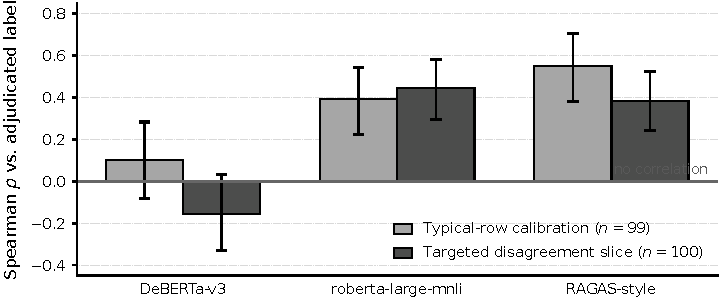
\includegraphics[width=0.62\linewidth]{figures/slice_dependent_ranking.pdf}
\caption{Scorer ranking against adjudicated humans is
slice-dependent: RAGAS-style leads on typical rows;
\texttt{roberta-large-mnli} leads on the disagreement slice, where
the legacy DeBERTa proxy turns weakly negative.
Error bars are bootstrap $95\%$ CIs.}
\label{fig:slice_ranking}
\end{figure}

\paragraph{Interpretation.}
Figure~\ref{fig:slice_ranking} makes the inversion visually obvious:
on the targeted disagreement slice \texttt{roberta-large-mnli} is the
strongest-aligned scorer (Spearman $\rho=0.446$, AUROC $0.794$,
AUPRC $0.929$); RAGAS-style is second ($\rho=0.384$, AUROC $0.718$);
the legacy DeBERTa proxy turns weakly negative ($\rho=-0.156$,
AUROC $0.398$). This is \emph{not} the typical-row ordering. We do
not claim any single scorer is universally best, and we do not treat
the $n=100$ slice as a population-level estimate. We treat the
typical-row calibration plus an adversarial disagreement probe as a
defensible minimum disclosure for this axis; finer protocols are an
open question.

\section{Threshold Transfer}
\label{sec:threshold_transfer}

Recovery is the dimensionless normalised contrast
$R_\tau(d) = \big(\mathrm{faith}_{\mathrm{gate},\tau}(d) -
\mathrm{faith}_{\mathrm{v1}}(d)\big) \big/
\big(\mathrm{faith}_{\mathrm{base}}(d) -
\mathrm{faith}_{\mathrm{v1}}(d)\big)$;
\textbf{values can exceed $1$ or be negative when the
no-refinement$-$aggressive-refinement denominator is small or
sign-inverted}, so the table is a transport diagnostic, not a
universal utility score. A faithfulness claim that depends on a tuned
operating threshold $\tau$ should report whether $\tau$ transfers
across datasets. We sweep $\tau \in \{0.3, 0.4, 0.5, 0.6, 0.7\}$ for
a CCS-gate retrieval intervention. For each tune dataset, $\tau^\ast$
is the threshold that maximises recovery on that dataset alone;
diagonal recovery evaluates $\tau^\ast$ on the same dataset, while
off-diagonal recovery evaluates it on the four other datasets.

\begin{table}[!htb]
\centering
\caption{Threshold transfer summary. For each tune dataset, $\tau^\ast$
is the value of $\tau$ that maximises recovery on that dataset alone;
``diagonal recovery'' is recovery at $\tau^\ast$ on the same dataset;
``off-diagonal mean'' is the mean recovery at $\tau^\ast$ over the four
\emph{other} eval datasets. A large positive gap means the tuned
$\tau^\ast$ does not transport. The full per-cell transfer matrix is
in supplement \S 11.}
\label{tab:threshold_transfer_main}
\footnotesize
\begin{tabular}{lcrrr}
\toprule
$\tau$ tuned on & $\tau^\ast$ & Diagonal recovery & Off-diagonal mean & Gap (diag $-$ off-diag) \\
\midrule
PubMedQA  & $0.4$ & $+1.452$ & $+0.451$ & $+1.002$ \\
NaturalQs & $0.5$ & $+1.401$ & $+0.211$ & $+1.191$ \\
SQuAD     & $0.3$ & $+0.823$ & $-0.141$ & $+0.963$ \\
TriviaQA  & $0.4$ & $+0.464$ & $+0.698$ & $-0.234$ \\
HotpotQA  & $0.3$ & $-0.112$ & $+0.093$ & $-0.205$ \\
\bottomrule
\end{tabular}
\end{table}

Tune-SQuAD and tune-HotpotQA both pick $\tau^\ast = 0.3$, and
tune-PubMedQA and tune-TriviaQA both pick $\tau^\ast = 0.4$, so the
off-diagonal columns coincide for those tune-dataset pairs in the
full $5{\times}5$ matrix (supplement \S 9); this is a faithful
consequence of the experiment, not a duplicate-row bug.

\paragraph{Interpretation.} PubMedQA, NaturalQuestions, and SQuAD
show a positive diagonal-vs-off-diagonal gap large enough to flag:
tuning $\tau$ on one of them and transporting it loses most of the
on-diagonal normalised contrast. The transfer table contains
sign-changing cells, which is the load-bearing finding for the
threshold axis.

% Section 10 (Coherence vs.\ Generic Retrieval Noise) lives in the
% supplement (\S 10) for the 9-page body limit; one
% sentence in \S\ref{sec:discussion} carries the headline.

\section{Cost-Aware Baselines}
\label{sec:cost}

Faithfulness numbers reported without latency and indexing cost are
under-identified along the cost axis. This section is not a leaderboard;
it is an identifiability test for deployment claims. We re-run a
head-to-head on $n=200$ SQuAD and $n=200$ HotpotQA queries with three
baselines: CRAG~\citep{yan2024crag}, gated-refinement (HCPC-v$2$),
and a $2$-level RAPTOR~\citep{raptor2024} index.

\begin{table}[!htb]
\centering
\caption{Cost-aware head-to-head, $n=200$ per (dataset, condition).
Latency is end-to-end per query; indexing time is the offline cost
of building the dataset's retrieval structure. Faithfulness CIs are
bootstrap $95\%$ intervals; hallucination CIs are Wilson $95\%$
intervals. RAPTOR-$2$L's indexing cost is $17$--$22\times$ the
dense-baseline ($n=200$ per cell).}
\label{tab:cost_main}
\scriptsize
\begin{tabular}{llcccc}
\toprule
Dataset & Condition & Faithfulness & Hallucination & Mean latency & Indexing \\
\midrule
SQuAD    & CRAG                       & $0.698\,[0.675,0.722]$ & $12.0\%\,[8.2,17.2]$  & $1{,}440$ ms & $\phantom{1}8.0$ s \\
SQuAD    & gated-refinement (HCPC-v$2$) & $0.708\,[0.685,0.732]$ & $12.5\%\,[8.6,17.8]$  & $1{,}720$ ms & $\phantom{1}8.0$ s \\
SQuAD    & RAPTOR-$2$L                & $0.710\,[0.685,0.735]$ & $12.5\%\,[8.6,17.8]$  & $1{,}714$ ms & $175.4$ s \\
HotpotQA & CRAG                       & $0.643\,[0.627,0.658]$ & $10.5\%\,[7.0,15.5]$  & $1{,}941$ ms & $\phantom{1}8.0$ s \\
HotpotQA & gated-refinement (HCPC-v$2$) & $0.633\,[0.617,0.650]$ & $12.5\%\,[8.6,17.8]$  & $2{,}289$ ms & $\phantom{1}8.0$ s \\
HotpotQA & RAPTOR-$2$L                & $0.631\,[0.615,0.647]$ & $13.0\%\,[9.0,18.4]$  & $2{,}414$ ms & $134.0$ s \\
\bottomrule
\end{tabular}
\end{table}

\paragraph{Harness and cost accounting.} This is a closed,
zero-dollar local/free-tier harness: local Ollama/Mistral generation,
Chroma indexing, MiniLM cross-encoders, no paid APIs. The CRAG
reimplementation uses the documented evaluator/strip-refinement
structure with live web search disabled, so its external-call count
is zero. A live-web CRAG would need to report web-call count, API
cost, and network latency separately. Self-RAG~\citep{asai2024selfrag}
is reported only in the supplement because its reflective decoding
violates the fixed-context assumption.

At $n=200$ per cell, faithfulness differences are inside CI overlap
and the only axis with non-overlapping ranges is indexing cost
($17$--$22\times$ for RAPTOR-$2$L). The cost axis is therefore the
only axis that produces a defensible ranking on this cell, and
ControlledRAG asks for it to be reported alongside the faithfulness
table.

\section{Discussion}
\label{sec:discussion}

\paragraph{What survives, by axis.} Strength tags reflect evidence
weight on this audit, not effect size.
\begin{itemize}\setlength{\itemsep}{0pt}\setlength{\parsep}{0pt}\setlength{\topsep}{2pt}
\item \emph{Generator} \textbf{[WEAK]}: second-generator probe
  (Qwen$2.5$, $n=100$, one model) preserves the metric-fragility
  ordering; not a panel claim.
\item \emph{Retriever} \textbf{[MEDIUM]}: matched HIGH$>$LOW CCS
  preserved across MiniLM/BGE/E5 (supp.\ \S 4); fixed generations
  unchanged.
\item \emph{Context structure} \textbf{[STRONG]}: matched CCS
  intervention null ($-0.002$, paired Wilcoxon $p=0.628$); span and
  CCS are complementary diagnostic axes.
\item \emph{Scorer} \textbf{[STRONG]}: raw contrasts
  $0.011 / 0.032 / 0.140$ on the same fixed generations;
  context-conditioned NLI sign-flips both backbones with disjoint
  bootstrap CIs (\S\ref{sec:metric_fragility}).
\item \emph{Human calibration} \textbf{[STRONG]}:
  $n=99$ ($\kappa=0.774$) ranks RAGAS-style first;
  $n=100$ ($\kappa=0.721$) ranks \texttt{roberta-large-mnli} first
  and the legacy DeBERTa proxy weakly negative. Slice-dependent.
\item \emph{Threshold} \textbf{[MEDIUM]}: $5{\times}5$ transfer
  table has sign-changing cells; no bootstrap CIs.
\item \emph{Cost} \textbf{[WEAK]}: faithfulness CIs overlap at
  $n=200$; the indexing-cost gap ($17$--$22\times$ for RAPTOR-$2$L)
  is the clear signal.
\end{itemize}
Coherence-preserving and random-noise slopes differ in point
estimate, but no significance test was run; see supplement
\S 10. Scope limits on the empirical demonstration are
categorised in \S\ref{sec:limits}.

\paragraph{The seven axes are load-bearing in different proportions.}
ControlledRAG asks for all seven to be reported because
under-identification on any single one can move the headline; the
weight of evidence on a given axis (the \textbf{[STRONG]} /
\textbf{[MEDIUM]} / \textbf{[WEAK]} tags above) reflects this audit,
not a property of the standard. In this audit, all seven axes are
load-bearing, but in different proportions.

\section{Limitations and Ethics}
\label{sec:limits}

\paragraph{Audited surface.} Audited cells are mostly short-answer
extractive QA on SQuAD with $7$B-class generators; the matched-context
audit is SQuAD-only; the long-form QASPER/MS-MARCO probe has $40$
distinct questions and is supplement-only.
Self-RAG~\citep{asai2024selfrag} runs in a harness mismatched with
the audit's fixed-context protocol and is supplement-only. Stronger
embeddings preserve the matched HIGH$>$LOW CCS ordering, but the
fixed-generation null is unchanged.

\paragraph{Human evaluation.} The typical-row calibration ($n=99$)
has overlapping bootstrap CIs across scorers; the targeted
disagreement slice ($n=100$) is adversarial-by-construction. Both
arms rest on two raters plus adjudication, not a broad annotator
pool, and neither slice settles a global scorer order. The
slice-dependence of the ranking is the load-bearing finding.

\paragraph{Scope of replication.} The second-generator probe is one
local Qwen$2.5$ model at $n=100$ fixed contexts per condition (a
sanity check, not a panel replication); the context-conditioned NLI
rescoring is on a $n=600$ balanced subset, not the full $7{,}500$
(sufficient to demonstrate input-format sign-flipping, not a
full-table replacement).

\paragraph{Ethics.} Public datasets and free-tier or local compute
only; the annotation arms cover short-answer support judgments on
public content (no PII, no sensitive content); annotator identities
are not stored. Review artifact anonymized; public links follow
acceptance.

\noindent These limits narrow the breadth of the empirical
demonstration but do not threaten the methodological claim, because
the seven-axis decomposition is motivated by the disclosure
principle in \S\ref{sec:controlledrag} and not by any single
empirical cell.

% The conclusion is folded into the §1 contributions block and the
% §12 by-axis bullets to keep the body within the 9-page limit. The
% standalone "Conclusion" section was removed because it duplicated
% content already in the abstract and §12.
